\chapter{Lecture 10: Einstein's Equation, Wave Motion, and the Cosmological Constant}

This lecture advances by a sequence of deliberate reductions. We begin with the simplest possible geometric question: empty flat space, then one particle, then the problem of finding a geometry that is flat everywhere except at one point. That low-dimensional warm-up is not a digression. It sets up the claim that dimension matters physically. From there the lecture turns to the algebraic form of Einstein's equation, pauses to ask what status that equation really has, and then makes a very characteristic move: before solving Schwarzschild, we go back to principle and ask how one promotes familiar special-relativistic equations into generally covariant form. That route leads to a scalar wave equation, to a scalar-field stress-energy tensor, and then back out into pressure, shear, localized sources, asymptotic flatness, and the cosmological constant. These notes follow Leonard Susskind closely, and where the blackboard arrangement carries part of the reasoning we keep the LazyingArt LLC and Video2Book evidence nearby rather than polishing it away.

\section{Conical Gravity and a Dimensional Warm-Up}

The lecture begins almost theatrically: here is space; let us concentrate on space. If there is no energy around, spacetime may be taken to be flat, and a constant-time slice is just an ordinary flat space. Now put a particle into it. The right-hand side of Einstein's equation is no longer zero where the particle sits, and so we ask the classroom question that sets the whole lecture in motion:

What geometry is flat everywhere except at one point?

The answer comes back immediately: a cone. In \(2+1\) dimensions the gravitational field of a point mass is not introduced as a \(1/r\) potential. Instead, space itself is flat away from the source, but with a conical deficit at the source. Time is simply carried along: one may picture time running upward while each spatial slice is a cone.

The lecture only needs the proportionality
\begin{equation}
\delta \propto m,
\end{equation}
for the deficit angle \(\delta\). It never stops to write the precise coefficient, so we should not manufacture one. The important point is that zero mass means zero deficit, and more mass means a larger missing wedge.

That conclusion is also robust under smoothing. The source need not be an ideal point particle. If the energy is distributed through a bounded region, the geometry need not be exactly conical at the center, but outside the source region it asymptotes to the same cone. One may round off the tip, but the exterior still remembers the total deficit.

\begin{figure}
\centering
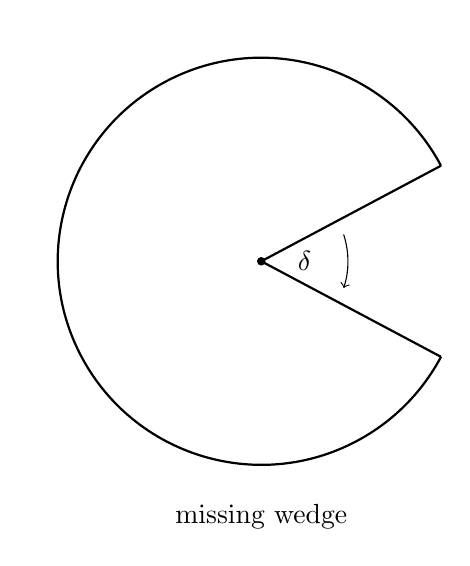
\begin{tikzpicture}[scale=1.1]
\draw[thick] (0,0) -- (28:2.35);
\draw[thick] (0,0) -- (332:2.35);
\draw[thick] (28:2.35) arc[start angle=28,end angle=332,radius=2.35];
\draw[->] (18:1.0) arc[start angle=18,end angle=-18,radius=1.0];
\node at (0.5,0) {\(\delta\)};
\fill (0,0) circle (1.4pt);
\node at (0,-2.95) {missing wedge};
\end{tikzpicture}
\caption{Transcript reconstruction of the conical deficit. Away from the tip the geometry is flat; the mass is encoded in the missing angle \(\delta\).}
\end{figure}

Susskind then extracts the physical lesson. If the deficit angle keeps growing with mass, what happens when it reaches \(360^\circ\)? The cone closes up. There is no opening left. In this way the lecture argues that low-dimensional gravity is too cramped to support much structure. One does not get a spacious world full of long-lived gravitating systems; one gets a geometry that can close up altogether.

That is why the conical picture belongs at the beginning. It shows, in one stroke, how a localized source can produce localized curvature and why the number of dimensions is not mere notation.

\section{Why \(3+1\) and Why Time Counts as a Dimension}

Having used the cone to rule out too little space, the lecture turns to ruling out too much. The discussion is qualitative, but the motivation is sharp. In more than three spatial dimensions the force law steepens. At the level of this lecture, the reliable point is simply the comparison
\begin{equation}
F(r)\sim r^{-2},\qquad r^{-3},\qquad r^{-4},
\end{equation}
as the number of spatial dimensions rises from three to four to five. The transcript is garbled in the plotted comparison, but the physical use of the comparison is unambiguous: higher-dimensional forces are more singular at short distances and less effective at holding extended structure together at large distances.

For gravity this means unstable orbital motion. Solar systems become chaotic. Planets are too easily ejected. For electromagnetism the same scaling is disastrous for atoms. The outer electrons are too weakly bound, while the inner attraction becomes too severe. Chemistry disappears. The lecture even pushes the point further: if electromagnetic binding fails this way, then the strong interactions would also be badly distorted. So the case for \(3+1\) is not that four dimensions are mathematically sacred, but that basic physics becomes thorny and unstable elsewhere.

The lecture also fields a question about more than one time dimension and refuses to pretend that this is merely another variant to classify. The answer is that it is too confusing to think about profitably at this stage. That refusal is part of the method: the lecture keeps hold of what can be visualized and calculated, and postpones what merely dazzles.

\subsection{Question \& Answer}

\paragraph{Question.} Why does time deserve dimensional status?

\paragraph{Answer.} Because special relativity mixes space and time together. That is the lecture's answer, and it is a good one. In Newtonian mechanics one thinks of time as external, a universal parameter. In special relativity that is no longer natural. Lorentz transformations mix space and time in a way that mathematically resembles rotations, except for the signature.

With our convention,
\begin{equation}
\eta_{\mu\nu}=\mathrm{diag}(1,-1,-1,-1),
\end{equation}
so time is not on exactly the same footing as space. But it is one coordinate direction of spacetime, not something outside the coordinate system. There is no unique time axis once we allow different inertial observers. A moving frame has a different time direction and a correspondingly tilted set of spatial directions.

The lecture's preferred way to say this is operational: boosts mix space and time, and in the same way energy and momentum mix as components of a four-vector. Once that becomes the language of the physics, it becomes natural to speak of four-dimensional spacetime.

\section{Einstein's Equation, Covariant Conservation, and the \(\lambda\) Ambiguity}

A student now asks where the cosmological constant goes. Susskind answers in a characteristic order: the more interesting question is what the cosmological constant does, but first we must decide where it belongs in the equation.

On the right-hand side sits the energy-momentum tensor \(T_{\mu\nu}\), so the left-hand side must also be a two-index tensor. The simplest geometric candidates are \(R_{\mu\nu}\) and \(g_{\mu\nu}R\). Indices may be raised or lowered as needed; what matters is the tensor structure. So we are led to consider
\begin{equation}
R_{\mu\nu}+c\,g_{\mu\nu}R,
\end{equation}
with the coefficient \(c\) still to be fixed.

It is fixed by conservation. If energy and momentum are conserved, then in covariant language
\begin{equation}
\nabla_\mu T^{\mu\nu}=0.
\end{equation}
The left-hand side of Einstein's equation must satisfy the same sort of identity. The correct linear combination is the Einstein tensor,
\begin{equation}
G_{\mu\nu}\equiv R_{\mu\nu}-\frac12 g_{\mu\nu}R,
\end{equation}
and the crucial property is
\begin{equation}
\nabla_\mu G^{\mu\nu}=0.
\end{equation}

That is the first main algebraic hinge of the lecture: the coefficient \(\frac12\) is not decorative. It is what makes the geometric side covariantly conserved for arbitrary geometry.

\begin{figure}
\centering

\includegraphics[width=0.62\textwidth]{lecture_10_figure_02.png}
\caption{Covariant conservation and metric compatibility on the board.}
\end{figure}

The board then adds the second equation that matters:
\begin{align}
\nabla_\mu G^{\mu\nu} &= 0, \\
\nabla_\mu g^{\mu\nu} &= 0.
\end{align}
The visual pairing is important. The lecture is not merely listing two facts. It is showing why the second fact opens the door to the cosmological constant.

Since the covariant derivatives of the metric vanish, we are free to add a term proportional to the metric itself without spoiling covariant conservation. Thus the equation becomes
\begin{equation}
R_{\mu\nu}-\frac12 g_{\mu\nu}R+\lambda g_{\mu\nu}=k\,T_{\mu\nu}.
\end{equation}
This \(\lambda\) is the cosmological constant. At this point the lecture does not yet linger on cosmology. It only insists that the ambiguity is real, and that Einstein discovered it from the mathematical structure of the equations themselves.

\subsection{Question \& Answer}

\paragraph{Question.} Why may we add \(\lambda g_{\mu\nu}\) without spoiling conservation?

\paragraph{Answer.} Because the metric is covariantly constant. The lecture gives a local geometric explanation. At any chosen point \(P\), one may adopt coordinates in which
\begin{equation}
g_{\mu\nu}(P)=\eta_{\mu\nu},
\qquad
\partial_\alpha g_{\mu\nu}(P)=0.
\end{equation}
At that point the Christoffel symbols vanish, so the covariant derivative of the metric vanishes there as well. Since \(\nabla_\alpha g_{\mu\nu}\) is itself a tensor, if it vanishes in one coordinate system at that point, it vanishes in every coordinate system at that point. Thus
\begin{equation}
\nabla_\alpha g_{\mu\nu}=0
\end{equation}
everywhere.

That is the whole mechanism. The Einstein tensor is covariantly conserved, and the metric is covariantly conserved, so the combination \(G_{\mu\nu}+\lambda g_{\mu\nu}\) is covariantly conserved too.

The lecture immediately appends a physical remark. The cosmological constant does not look like a small correction to the inverse-square law. In the Newtonian analogy it produces a force proportional to distance. So even before we analyze cosmology properly, we already know that \(\lambda\) represents a genuinely different sort of gravitational behavior.

\section{Newtonian Limit and the Status of Einstein's Guess}

The lecture now steps back and asks a methodological question: was Einstein's equation derived from first principles? The answer is no. The equation is a guess, though not an arbitrary one. It is a tensorial guess, constrained by covariance and by the requirement that it reproduce Newtonian gravity in the appropriate limit.

Take the \(00\)-component of Einstein's equation in the regime of weak fields and slow motions. On the right-hand side, the dominant contribution is the energy density,
\begin{equation}
T_{00}\approx \rho.
\end{equation}
On the left-hand side, if the geometry is close to flat and static, the lecture says that one finds something proportional to a purely spatial second derivative of \(g_{00}\). In cautious form,
\begin{equation}
\nabla^2 g_{00}\propto \rho,
\end{equation}
with the explicit lecture-level warning that the factor of two is easy to miss.

Now \(g_{00}\) is closely related to the Newtonian potential \(\Phi\). So the \(00\)-component reduces to the Poisson equation,
\begin{equation}
\nabla^2\Phi=4\pi G\,\rho.
\end{equation}
That is the correspondence principle at work.

Susskind is careful here. Einstein did not prove from logic alone that the equations must take this form. He insisted that the equations should have the same form in every reference frame, and then looked for a tensor equation that reduced to Newton in the weak, static regime. The success of the theory is then empirical. In ordinary weak fields it agrees with Newton where it must. In strong fields and at high speeds it departs from Newton, and experiment sides with Einstein.

This is an important beat in the lecture. Without it, the derivation of the left-hand side would sound too self-contained. With it, the equation recovers its proper status: a brilliantly constrained physical guess.

\section{Equivalence Principle as a Recipe: From Flat-Space Waves to Curved-Space Waves}

Before studying Schwarzschild, the lecture makes another deliberate detour. Rather than jumping into solutions, it asks how modern physicists use the equivalence principle. The answer is not mystical. It is procedural.

In a sufficiently small region of spacetime, curvature cannot be detected. In such a region one may choose coordinates in which the metric looks Minkowskian and its first derivatives vanish at the point. Then the equations of physics should take the same form they take in special relativity. The lecture compares this to a small patch on the surface of the Earth: on the right scale it looks flat.

\begin{figure}
\centering
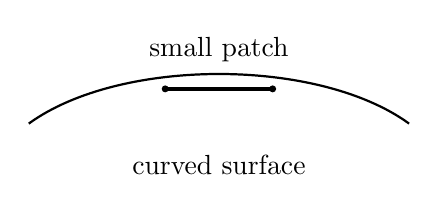
\begin{tikzpicture}[scale=1.05]
\draw[thick] (-2.3,0) .. controls (-1.2,0.8) and (1.2,0.8) .. (2.3,0);
\draw[very thick] (-0.65,0.42) -- (0.65,0.42);
\fill (-0.65,0.42) circle (1.2pt);
\fill (0.65,0.42) circle (1.2pt);
\node at (0,0.9) {small patch};
\node at (0,-0.5) {curved surface};
\end{tikzpicture}
\caption{Transcript reconstruction of local flatness. On a sufficiently small patch, curvature is not detectable and the flat-space equations apply.}
\end{figure}

That principle is then turned into a recipe. If we know a law in special relativity, we rewrite it as a tensor equation. Once it has genuine tensor form, we may carry that same equation over into curved spacetime.

The lecture briefly reminds us that this is how geodesic motion arose. A free particle in flat spacetime moves in a straight line. In curved spacetime it moves along the straightest possible line, namely a geodesic. The new example is wave motion.

Begin with the simplest wave equation in one spatial dimension:
\begin{equation}
\partial_t^2\phi=c^2\,\partial_x^2\phi.
\end{equation}
To describe propagation in three spatial dimensions we add the other second derivatives:
\begin{equation}
\partial_t^2\phi
=
c^2\left(\partial_x^2+\partial_y^2+\partial_z^2\right)\phi.
\end{equation}
Now set \(c=1\) and write the result in Minkowski notation:
\begin{equation}
\eta^{\mu\nu}\partial_\mu\partial_\nu\phi=0.
\end{equation}
This is where the lecture deliberately creates tension. We have written the wave equation in a form that looks covariant. But looks are not enough.

\subsection{Question \& Answer}

\paragraph{Question.} Why is \(g^{\mu\nu}\partial_\mu\partial_\nu\phi=0\) not yet a tensor equation?

\paragraph{Answer.} Because replacing \(\eta^{\mu\nu}\) by \(g^{\mu\nu}\) still leaves ordinary derivatives acting where covariant derivatives are required. The derivative of a scalar, \(\partial_\nu\phi\), is a vector. Raising its index with the metric gives another vector, \(g^{\mu\nu}\partial_\nu\phi\). But differentiating a vector with an ordinary derivative does not yield a tensor.

So the corrected equation is
\begin{equation}
\nabla_\mu\!\left(g^{\mu\nu}\partial_\nu\phi\right)=0.
\end{equation}
Now the equation is genuinely covariant.

The lecture then pauses over the Leibniz rule because a student asks for it explicitly. Covariant derivatives obey
\begin{equation}
\nabla_\mu(AB)=(\nabla_\mu A)B+A(\nabla_\mu B).
\end{equation}
Applying this and using metric compatibility gives
\begin{align}
\nabla_\mu\!\left(g^{\mu\nu}\partial_\nu\phi\right)
&=
(\nabla_\mu g^{\mu\nu})\partial_\nu\phi
+
g^{\mu\nu}\nabla_\mu\nabla_\nu\phi \\
&=
g^{\mu\nu}\nabla_\mu\nabla_\nu\phi,
\end{align}
because \(\nabla_\mu g^{\mu\nu}=0\). Therefore the wave equation may also be written as
\begin{equation}
\nabla_\mu\nabla^\mu\phi=0.
\end{equation}

This is the cleaned tensor formula, but the lecture's false starts are pedagogically useful. They show exactly where the promotion from flat-space notation to curved-space notation becomes nontrivial. One does not merely swap \(\eta\) for \(g\); one must preserve the transformation properties of the whole expression.

The physical reading follows immediately. Once the Christoffel symbols enter the equation, the gravitational field is acting directly on the wave. The coefficients of the wave equation become position-dependent. That is why the lecture compares curved spacetime to a variable medium such as a material with changing density or dielectric constant. The safe claim, and the only one we need here, is that the wave bends and its propagation is altered by the position dependence of the geometry.

\section{Closing the System: The Scalar-Field Stress-Energy Tensor}

At this point the lecture reverses the arrow of explanation. We have seen how gravity affects the wave field. Now we ask what belongs on the right-hand side if the wave field itself is to source gravity.

Again Susskind starts in flat spacetime. There we know the scalar wave equation,
\begin{equation}
\eta^{\mu\nu}\partial_\mu\partial_\nu\phi=0.
\end{equation}
We want a two-index tensor built out of \(\phi\). The simplest indexed objects come from derivatives of \(\phi\), so a natural ansatz is
\begin{equation}
T_{\mu\nu}
=
\partial_\mu\phi\,\partial_\nu\phi
+
C\,\eta_{\mu\nu}\,\partial_\sigma\phi\,\partial^\sigma\phi.
\end{equation}
The lecture's first filter is physical, not formal. Energy should not change sign when \(\phi\) is replaced by \(-\phi\). A wave and the same wave with opposite sign are not physically opposite-energy states. They are like the two sides of a harmonic oscillation. So the stress tensor should be quadratic in the field.

The coefficient \(C\) is then fixed by conservation. We want
\begin{equation}
\partial^\mu T_{\mu\nu}=0
\end{equation}
for fields satisfying the wave equation. The calculation goes exactly the way the lecture sketches it on the board.

\begin{enumerate}
\item Differentiate the first term:
\begin{align}
\partial^\mu\!\left(\partial_\mu\phi\,\partial_\nu\phi\right)
&=
(\partial^\mu\partial_\mu\phi)\partial_\nu\phi
+
(\partial^\mu\phi)(\partial_\mu\partial_\nu\phi).
\end{align}

\item The first contribution vanishes by the wave equation.

\item Differentiate the second term:
\begin{align}
\partial^\mu\!\left(\eta_{\mu\nu}\,\partial_\sigma\phi\,\partial^\sigma\phi\right)
&=
\partial_\nu\!\left(\partial_\sigma\phi\,\partial^\sigma\phi\right) \\
&=
2\,(\partial^\sigma\phi)(\partial_\nu\partial_\sigma\phi).
\end{align}

\item Since ordinary derivatives commute in flat spacetime, this has the same index structure as the remaining term from step 1. Therefore the two pieces cancel provided
\begin{equation}
C=-\frac12.
\end{equation}
\end{enumerate}

So the tensor is
\begin{equation}
T_{\mu\nu}
=
\partial_\mu\phi\,\partial_\nu\phi
-
\frac12\eta_{\mu\nu}\,\partial_\alpha\phi\,\partial^\alpha\phi.
\end{equation}
This is the canonical flat-space scalar-field stress-energy tensor, and it matches the legible board equation.

\begin{figure}
\centering

\includegraphics[width=0.86\textwidth]{lecture_10_figure_03.png}
\caption{Scalar-field stress-energy tensor and the \(T_{00}\) energy density on the board.}
\end{figure}

The lecture then asks for the component we care most about first, namely the energy density. With \(\mu=\nu=0\), and using the signature \((+---)\), we obtain
\begin{align}
T_{00}
&=
\dot{\phi}^{\,2}
-
\frac12\left[
\dot{\phi}^{\,2}
-
\left(\frac{\partial\phi}{\partial x}\right)^2
-
\left(\frac{\partial\phi}{\partial y}\right)^2
-
\left(\frac{\partial\phi}{\partial z}\right)^2
\right] \\
&=
\frac12\left[
\dot{\phi}^{\,2}
+
\left(\frac{\partial\phi}{\partial x}\right)^2
+
\left(\frac{\partial\phi}{\partial y}\right)^2
+
\left(\frac{\partial\phi}{\partial z}\right)^2
\right].
\end{align}
The lecture insists on recognizing this, not merely writing it. The \(\dot{\phi}^{\,2}\) term is the kinetic energy density of the oscillating field. The spatial derivative terms are the stored elastic or gradient energy. The violin-string analogy belongs here because it tells us how to read the formula physically.

There is still one overall normalization ambiguity, but only one. Multiplying the whole tensor by a constant is equivalent to rescaling the field \(\phi\). So once the relative coefficient \(-\frac12\) has been fixed, the tensor is unique up to the conventional normalization of the field itself.

\section{Pressure, Shear, Localized Sources, and the Cosmological Constant Revisited}

Once the scalar-field example is in hand, the lecture broadens its interpretation of the source. The key point is that Einstein's right-hand side is not merely mass density in disguise. It is the full local content of energy, momentum, pressure, and stress.

In an isotropic local rest frame we may write, in the convention used here,
\begin{equation}
T_{\mu\nu}=\mathrm{diag}(\rho,p,p,p).
\end{equation}
The off-diagonal components vanish in that idealized situation, and the diagonal spatial entries are the pressure. If the system is not isotropic, the spatial diagonal entries need not be equal, and off-diagonal terms appear. Those off-diagonal components represent shear stresses. The lecture even remarks that a shear stress can be reinterpreted, after a \(45^\circ\) rotation, as unequal diagonal stretching and squeezing. That is why stress is a genuinely tensorial source and not just a scalar correction to mass density.

Later in the closing questions the lecture phrases the same idea more spectrally: one timelike eigenvalue corresponds to energy density in a comoving frame, while the spacelike eigenvalues describe the principal stresses. If the three spacelike eigenvalues coincide, the material is isotropic. If they differ, there are shear-like distortions or directional pressures.

\subsection{Question \& Answer}

\paragraph{Question.} If the source is localized, why is the field not zero elsewhere?

\paragraph{Answer.} Because a local equation does not imply a local support condition on its solutions. The lecture steps back to Newton for this:
\begin{equation}
\nabla^2\Phi=4\pi G\,\rho.
\end{equation}
If \(\rho\) vanishes outside the matter distribution, it does not follow that \(\Phi\) vanishes there. What vanishes there is the Laplacian. The solution still extends outward and gives the familiar exterior field.

The same logic carries into general relativity. \(T_{\mu\nu}\) can vanish away from the source, but the metric need not become trivial there. The field equation is pointwise, yet the solution is determined globally by matching and boundary behavior. That is why a localized mass produces a nontrivial exterior geometry.

The lecture uses this point to answer a related question about light. Since light carries energy and momentum, can light gravitate against light and therefore spoil perfect superposition? In principle yes. The schematic size is
\begin{equation}
F\sim G\,\frac{E_1E_2}{c^4\,r^2}.
\end{equation}
This already explains the practical answer. Because \(m=E/c^2\), the effective gravitational mass of an ordinary beam is tiny, and the interaction between ordinary light beams is negligible. So nonlinear gravitational interaction exists in principle, but not at an observable level for everyday light.

The lecture also gives a forward-looking remark: there is an unstable circular null orbit outside a black hole. We keep that statement qualitative here, because the exact radius belongs to the Schwarzschild analysis still to come.

\subsection{Question \& Answer}

\paragraph{Question.} Why does the cosmological constant not stabilize Einstein's static universe?

\paragraph{Answer.} First we recover the Newtonian analog. Up to a sign convention that the lecture itself treats loosely, a cosmological constant behaves like a uniform source spread through space. A convenient potential is
\begin{equation}
\Phi_\Lambda(\mathbf{x})
=
\frac{\lambda}{6}\left(x^2+y^2+z^2\right),
\end{equation}
since
\begin{equation}
\nabla^2\Phi_\Lambda=\lambda.
\end{equation}
Its gradient is linear:
\begin{equation}
\frac{\partial \Phi_\Lambda}{\partial x}=\frac{\lambda}{3}x,
\qquad
\frac{\partial \Phi_\Lambda}{\partial y}=\frac{\lambda}{3}y,
\qquad
\frac{\partial \Phi_\Lambda}{\partial z}=\frac{\lambda}{3}z.
\end{equation}
So the resulting force is proportional to distance. That is the hallmark of the cosmological term in the lecture. It is neither inverse-square nor centered on a distinguished origin in the ordinary sense. If everything recedes from everything else, every observer sees the same sort of expansion.

This already explains why the cosmological constant may live on either side of the equation. On the geometric side,
\begin{equation}
R_{\mu\nu}-\frac12 g_{\mu\nu}R+\lambda g_{\mu\nu}=k\,T_{\mu\nu},
\end{equation}
it is part of the geometry. On the matter side,
\begin{equation}
R_{\mu\nu}-\frac12 g_{\mu\nu}R
=
k\,T_{\mu\nu}-\lambda g_{\mu\nu},
\end{equation}
it may be read as a vacuum stress-energy present even when no ordinary matter is around. The lecture's joke is that \(\lambda\) is schizophrenic about which side it wants to inhabit. The mathematics allows both readings.

Einstein's historical mistake was not that he allowed the term. The mistake was that he hoped to use it to hold the universe in a stable static balance. The lecture makes the instability intuitive with an ordinary mechanical picture. Combine an attractive gravitational potential with the potential corresponding to a repulsive force proportional to distance. One can arrange a stationary point, but it is a maximum of the effective potential, not a minimum.

\begin{figure}
\centering
\begin{tikzpicture}[scale=1.0]
\draw[->] (-0.2,0) -- (5.5,0) node[right] {$r$};
\draw[->] (0,-3.15) -- (0,1.45) node[above] {$V(r)$};
\draw[thick] plot[smooth] coordinates {(0.8,-2.8) (1.1,-1.9) (1.6,-1.1) (2.3,-0.35) (3.0,0.18) (3.8,-0.15) (4.8,-1.5)};
\fill (3.0,0.18) circle (1.8pt);
\node[above] at (3.0,0.18) {unstable equilibrium};
\end{tikzpicture}
\caption{Transcript reconstruction of Einstein's static-universe balance. The tuned point is a maximum of the effective potential, so a small displacement drives the system away from equilibrium.}
\end{figure}

That is why the cosmological constant does not rescue a static universe. A delicate cancellation is possible, but it is an unstable armistice, not a stable resting point.

The lecture closes by separating several notions that are easy to confuse. Flat spacetime means no energy-momentum at all. Asymptotically flat spacetime is weaker: it means that far from localized sources the metric approaches Minkowski form,
\begin{equation}
g_{\mu\nu}\to \eta_{\mu\nu}
\qquad \text{as } r\to\infty.
\end{equation}
This is a statement about spacetime, not just about a spatial slice.

If \(\lambda\neq 0\), the far geometry is not asymptotically flat. In vacuum we have
\begin{equation}
R_{\mu\nu}-\frac12 g_{\mu\nu}R+\lambda g_{\mu\nu}=0.
\end{equation}
Contracting with \(g^{\mu\nu}\) in four dimensions gives
\begin{equation}
R-2R+4\lambda=0,
\end{equation}
so that, in the present sign convention,
\begin{equation}
R=4\lambda.
\end{equation}
The lecture explicitly wavers about the overall sign of \(\lambda\), so the invariant content matters more than the sign bookkeeping at this stage: a nonzero cosmological constant gives a nonzero uniform scalar curvature even in empty spacetime. The asymptotic geometry is then de Sitter or anti-de Sitter, not Minkowski.

The final classroom exchange sharpens the distinction once more. One must not confuse a nearly flat spatial geometry with a flat spacetime geometry. The real world is not exactly asymptotically flat, and that is precisely why cosmology must eventually enter the story.

\section{Summary}

The lecture begins with a cone and ends with a promise: next comes Schwarzschild. Between those two points it establishes a clear chain of ideas. First, low-dimensional geometry makes curvature local and visible, and immediately shows that dimension matters physically. Second, Einstein's equation is shaped by covariance and covariant conservation, but it still allows the extra \(\lambda g_{\mu\nu}\) term. Third, the equation is not a theorem of pure reason; it is a tensorial guess checked against Newton in the weak-field limit and then against experiment. Fourth, the equivalence principle gives us a working recipe: rewrite special-relativistic equations in genuine tensor form and then carry them into curved spacetime. Fifth, once we do that for a scalar wave, we can also build the corresponding stress-energy tensor and see explicitly that pressure and shear, no less than energy density, gravitate.

In Wheeler's condensed language, the lecture is teaching us that energy, momentum, pressure, and stress tell spacetime how to bend, while the metric and its Christoffel symbols tell matter and waves how to propagate. The natural next step is therefore the first great exact solution: the Schwarzschild metric, both as the field outside a spherical mass and as the geometry of a black hole.